\documentclass[14pt]{extreport}
\usepackage{cmap}
\usepackage[utf8]{inputenc}
\usepackage[english,ukrainian]{babel}
\usepackage{graphicx}
\usepackage{geometry}
\usepackage{listings}
\usepackage{amsmath}
\usepackage{float}
\geometry{
	a4paper,
	left=20mm,
	right=20mm,
	top=20mm,
	bottom=20mm
}
\lstset{
	columns=fullflexible, 
	frame=single, 
	breaklines=true, 
	tabsize=4,
	postbreak=\raisebox{0ex}[0ex][0ex]{\ensuremath{\hookrightarrow\space}},
	showstringspaces=false,% no symbol for spaces in strings
}
\graphicspath{ {./pictures} }
\setlength{\parindent}{4em}

\newcommand\subject{Бази даних}
\newcommand\lecturer{асистент кафедри ПЗ\\Білоіваненко М.В.}
\newcommand\teacher{асистент кафедри ПЗ\\Білоіваненко М.В.}
\newcommand\mygroup{ПЗ-32}
\newcommand\lab{10}
\newcommand\theme{Перетворення даних реляційної моделі у структуровані документи}
\newcommand\purpose{Перетворити дані реляційної моделі у структуровані документи}

\begin{document}
\begin{normalsize}
	\begin{titlepage}
		\thispagestyle{empty}
		\begin{center}
			\textbf{МІНІСТЕРСТВО ОСВІТИ І НАУКИ УКРАЇНИ\\
				НАЦІОНАЛЬНИЙ УНІВЕРСИТЕТ "ЛЬВІВСЬКА ПОЛІТЕХНІКА"}
		\end{center}
		\begin{flushright}
			Інститут \textbf{КНІТ}\\
			Кафедра \textbf{ПЗ}
		\end{flushright}
		\vspace{200pt}
		\begin{center}
			\textbf{ЗВІТ}\\
			\vspace{10pt}
			До лабораторної роботи № \lab\\
			\textbf{На тему}: “\textit{\theme}”\\
			\textbf{З дисципліни}: “\subject”
		\end{center}
		\vspace{40pt}
		\begin{flushright}
			
			\textbf{Лектор}:\\
			\lecturer\\
			\vspace{10pt}
			\textbf{Виконав}:\\
			
			студент групи \mygroup\\
			Коваленко Д.М.\\
			\vspace{10pt}
			\textbf{Прийняв}:\\
			
			\teacher\\
			
			\vspace{28pt}
			«\rule{1cm}{0.15mm}» \rule{1.5cm}{0.15mm} 2023 р.\\
			$\sum$ = \rule{1cm}{0.15mm}……………\\
			
		\end{flushright}
		\vspace{\fill}
		\begin{center}
			\textbf{Львів — 2023}
		\end{center}
	\end{titlepage}
		
	\begin{description}
		\item[Тема.] \theme.
		\item[Мета.] \purpose.
	\end{description}

	\section*{Лабораторне завдання}
Обрати формат структурованого представлення даних (JSON, XML або RDF). Розробити модель файлів для зберігання даних трьох зв’язаних сутностей предметної області.

На 3 бали: створити SQL-запити або збережені процедури, які експортують поточні дані обраних сутностей у вигляді документів встановленого формату. Використати спеціальні функції СУБД для побудови відповідних JSON- або XML-структур. 

На 6+ балів: обрати, встановити та налаштувати документну або графову СУБД. Завантажити до неї згенеровані файли із даними. Виконати декілька запитів на вибірку значень властивостей різних сутностей. Навести засоби з’єднання документів у запитах.	
	
	\section*{Хід роботи}
	\begin{figure}[H]
		\centering
		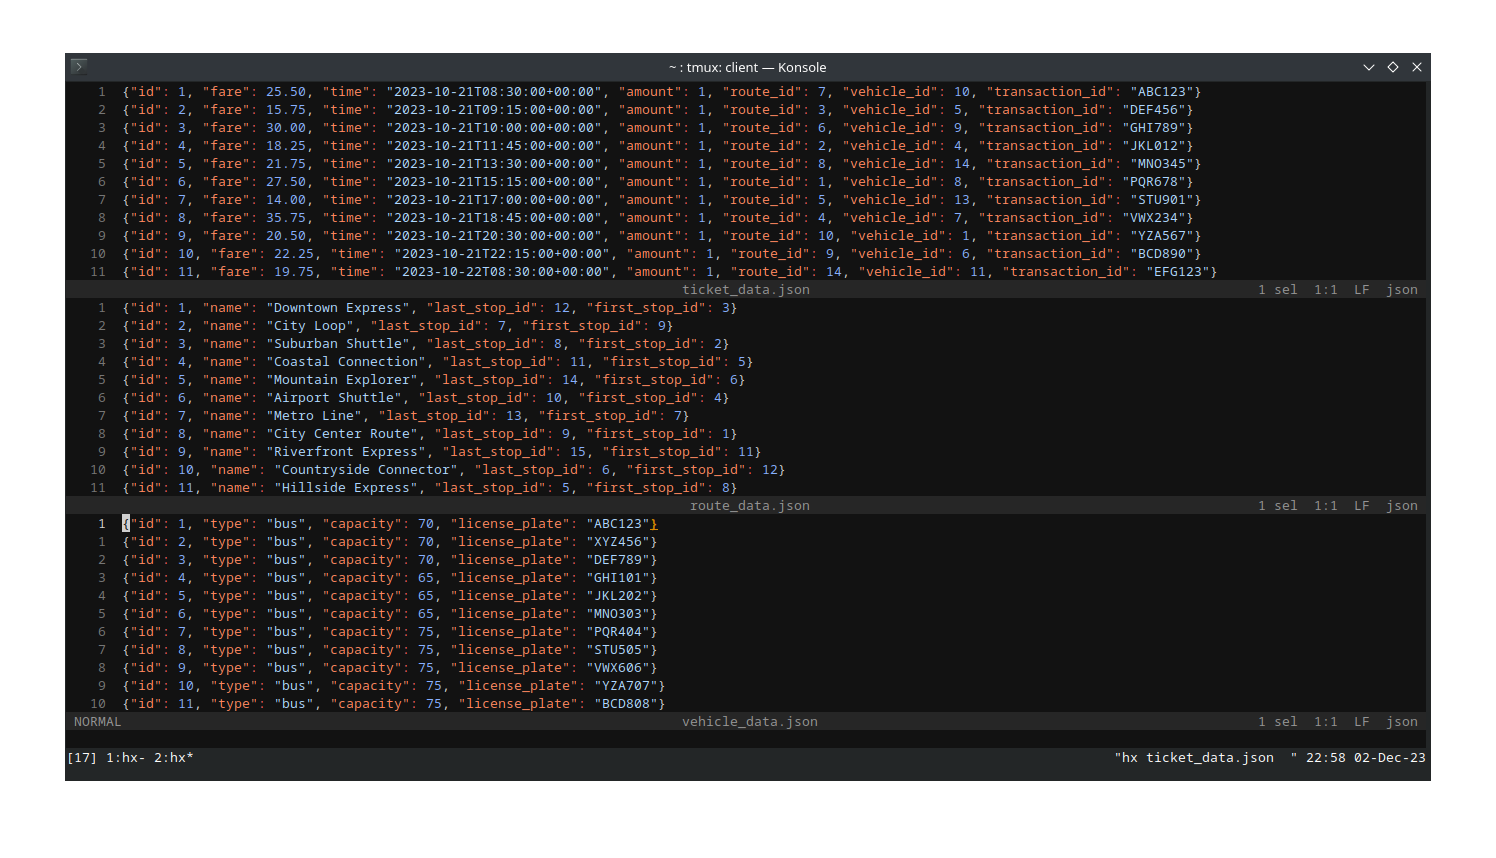
\includegraphics[scale=0.45]{1}
		\caption{Експортовані дані}
	\end{figure}
	
	\begin{lstlisting}[language=sql]
COPY (
SELECT jsonb_build_object(
	'id', id,
	'name', name,
	'first_stop_id', first_stop_id,
	'last_stop_id', last_stop_id
) AS route_json
FROM route
) TO '/var/lib/postgresql/data/route_data.json';

COPY (
SELECT jsonb_build_object(
	'id', t.id,
	'transaction_id', t.transaction_id,
	'fare', t.fare,
	'amount', t.amount,
	'time', t.time,
	'route_id', t.route_id,
	'vehicle_id', t.vehicle_id
) AS ticket_json
FROM ticket t
) TO '/var/lib/postgresql/data/ticket_data.json';

COPY (
SELECT jsonb_build_object(
	'id', id,
	'type', type,
	'license_plate', license_plate,
	'capacity', capacity
) AS vehicle_json
FROM vehicle
) TO '/var/lib/postgresql/data/vehicle_data.json';
	\end{lstlisting}
	
	\section*{Висновок}
	Під час виконання лабораторної роботи я створив SQL-запити, які експортують поточні дані обраних сутностей у вигляді документів встановленого формату. Використав спеціальні функції СУБД для побудови відповідних JSON- або XML-структур. 
	 
\end{normalsize}
\end{document}
